\chapter{Programación dinámica}
Partimos de una solución recursiva bruta y podemos hacer uso de una función de memorización. El ejemplo más clásico es el de Fibonacci
\section{Fibonacci}
\[
    fibonacci(n) = 
    \begin{cases*}
        0 & , $n = 0$ \\    
        1 & , $n = 1$ \\
        fibonacci( n - 1 ) + fibonacci( n - 2 ) & , $ n \geq 2$ 
    \end{cases*}    
\]

En código
\begin{lstlisting}
    int fibonacci( int n ){
        if( n == 0 )
            return 0;
        if( n == 1 )
            return 1;
        return fibonacci( n - 1 ) * fibonacci( n - 2 );
    }
\end{lstlisting}

Si dibujamos las llamadas recursivas como un árbol tenemos lo siguiente 

\begin{figure}[H]
    \begin{center}
        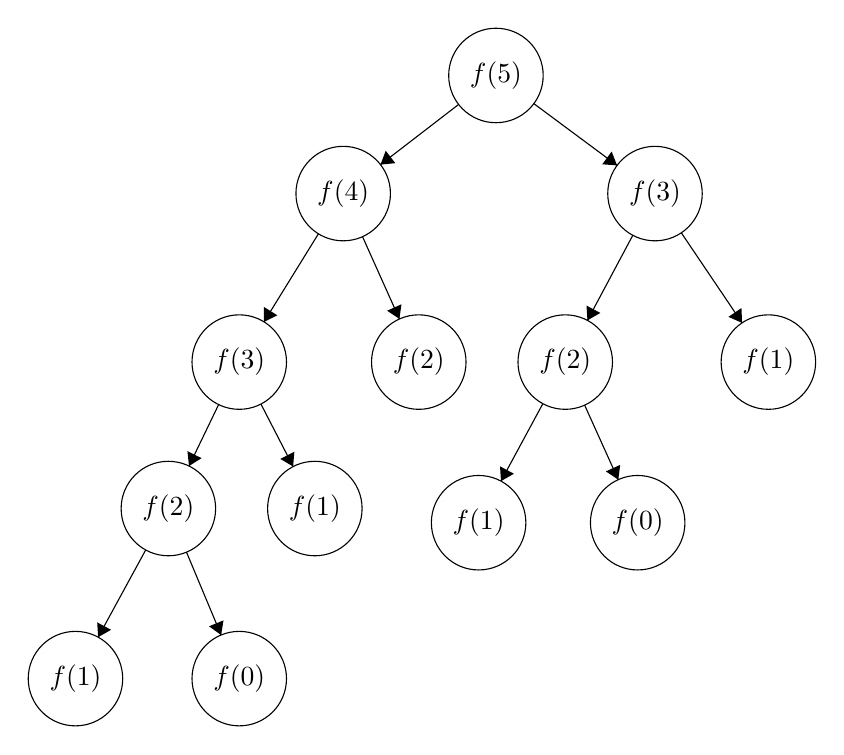
\begin{tikzpicture}[scale=0.2]
        \tikzstyle{every node}+=[inner sep=0pt]
        \draw [black] (38.5,-6.8) circle (3);
        \draw (38.5,-6.8) node {$f(5)$};
        \draw [black] (28.8,-14.3) circle (3);
        \draw (28.8,-14.3) node {$f(4)$};
        \draw [black] (48.6,-14.3) circle (3);
        \draw (48.6,-14.3) node {$f(3)$};
        \draw [black] (22.2,-25) circle (3);
        \draw (22.2,-25) node {$f(3)$};
        \draw [black] (33.6,-25) circle (3);
        \draw (33.6,-25) node {$f(2)$};
        \draw [black] (42.9,-25) circle (3);
        \draw (42.9,-25) node {$f(2)$};
        \draw [black] (55.8,-25) circle (3);
        \draw (55.8,-25) node {$f(1)$};
        \draw [black] (17.7,-34.3) circle (3);
        \draw (17.7,-34.3) node {$f(2)$};
        \draw [black] (27,-34.3) circle (3);
        \draw (27,-34.3) node {$f(1)$};
        \draw [black] (11.8,-45.1) circle (3);
        \draw (11.8,-45.1) node {$f(1)$};
        \draw [black] (22.2,-45.1) circle (3);
        \draw (22.2,-45.1) node {$f(0)$};
        \draw [black] (37.4,-35.2) circle (3);
        \draw (37.4,-35.2) node {$f(1)$};
        \draw [black] (47.5,-35.2) circle (3);
        \draw (47.5,-35.2) node {$f(0)$};
        \draw [black] (36.13,-8.64) -- (31.17,-12.46);
        \fill [black] (31.17,-12.46) -- (32.11,-12.37) -- (31.5,-11.58);
        \draw [black] (40.91,-8.59) -- (46.19,-12.51);
        \fill [black] (46.19,-12.51) -- (45.85,-11.63) -- (45.25,-12.44);
        \draw [black] (27.23,-16.85) -- (23.77,-22.45);
        \fill [black] (23.77,-22.45) -- (24.62,-22.03) -- (23.77,-21.5);
        \draw [black] (30.03,-17.04) -- (32.37,-22.26);
        \fill [black] (32.37,-22.26) -- (32.5,-21.33) -- (31.59,-21.74);
        \draw [black] (50.27,-16.79) -- (54.13,-22.51);
        \fill [black] (54.13,-22.51) -- (54.09,-21.57) -- (53.26,-22.13);
        \draw [black] (47.19,-16.95) -- (44.31,-22.35);
        \fill [black] (44.31,-22.35) -- (45.13,-21.88) -- (44.25,-21.41);
        \draw [black] (20.89,-27.7) -- (19.01,-31.6);
        \fill [black] (19.01,-31.6) -- (19.81,-31.1) -- (18.91,-30.66);
        \draw [black] (23.58,-27.67) -- (25.62,-31.63);
        \fill [black] (25.62,-31.63) -- (25.7,-30.69) -- (24.81,-31.15);
        \draw [black] (16.26,-36.93) -- (13.24,-42.47);
        \fill [black] (13.24,-42.47) -- (14.06,-42) -- (13.18,-41.53);
        \draw [black] (18.85,-37.07) -- (21.05,-42.33);
        \fill [black] (21.05,-42.33) -- (21.2,-41.4) -- (20.28,-41.78);
        \draw [black] (41.48,-27.64) -- (38.82,-32.56);
        \fill [black] (38.82,-32.56) -- (39.64,-32.09) -- (38.76,-31.62);
        \draw [black] (44.13,-27.73) -- (46.27,-32.47);
        \fill [black] (46.27,-32.47) -- (46.39,-31.53) -- (45.48,-31.94);
        \end{tikzpicture}
    \end{center}
\end{figure}

Como podemos observar hay llamadas recursivas que se repiten varias veces como ejemplo tenemos la llamada recursiva con un valor de 3, o 2. ¿Podemos evitar esto?

\begin{lstlisting}
    int memoria[ 100000 ];
    .
    .
    .
    int fibonacci( int n ){
        if( n == 0 )
            return 0;
        if( n == 1 )
            return 1;
        if( memoria[ n ] != -1 )
            return memoria[ n ];
        return memoria[ n ] = ( fibonacci( n - 1 ) * fibonacci( n - 2 ) );
    }

    int main(){
        memset( memoria, -1, sizeof(memoria) );
        .
        .
        .
    }
\end{lstlisting}

La complejidad la podemos calcular viendo los estados, en nuestro caso es el tamaño de la memoria, por ejemplo si llamamos a fibonacci de 10 siempre tenemos el mismo resultado, por tanto multiplicamos los estados por la complejidad de la función en nuestro caso es $10^{5} * constante$

\section{Coeficiente binomial}
\[
    Coef\_Bin(n, k) = 
    \begin{cases*}
        1 & , $n = k$ \\    
        1 & , $k = 0$ \\
        Coef\_Bin( n - 1, k - 1 ) + Coef\_Bin( n - 1, k ) & , $ k \leq n$ 
    \end{cases*}    
\]

Si programamos esta función tenemos lo siguiente: 

\begin{lstlisting}
    int coef_bin( int n, int k ){
        if( n == k || k == 0 )
            return 1;
        return ( coef_bin( n - 1, k - 1 ) + coef_bin( n - 1, k ) ); 
    }
\end{lstlisting}

Si aplicamos DP
\begin{lstlisting}
    memoria[ 1000 ][ 1000 ];
    int coef_bin( int n, int k ){
        if( n == k || k == 0 )
            return 1;
        if( mem[ n ][ k ] != -1 )
            return memoria[ n ][ k ];
        return memoria[ n ][ k ] = ( coef_bin( n - 1, k - 1 ) + coef_bin( n - 1, k ) ); 
    }
\end{lstlisting}
En complejidad tenemos $O(n * k)$ y sin la función de memorización tenemos $O(2^{n})$